\documentclass[main.tex]{subfiles}

\begin{document}

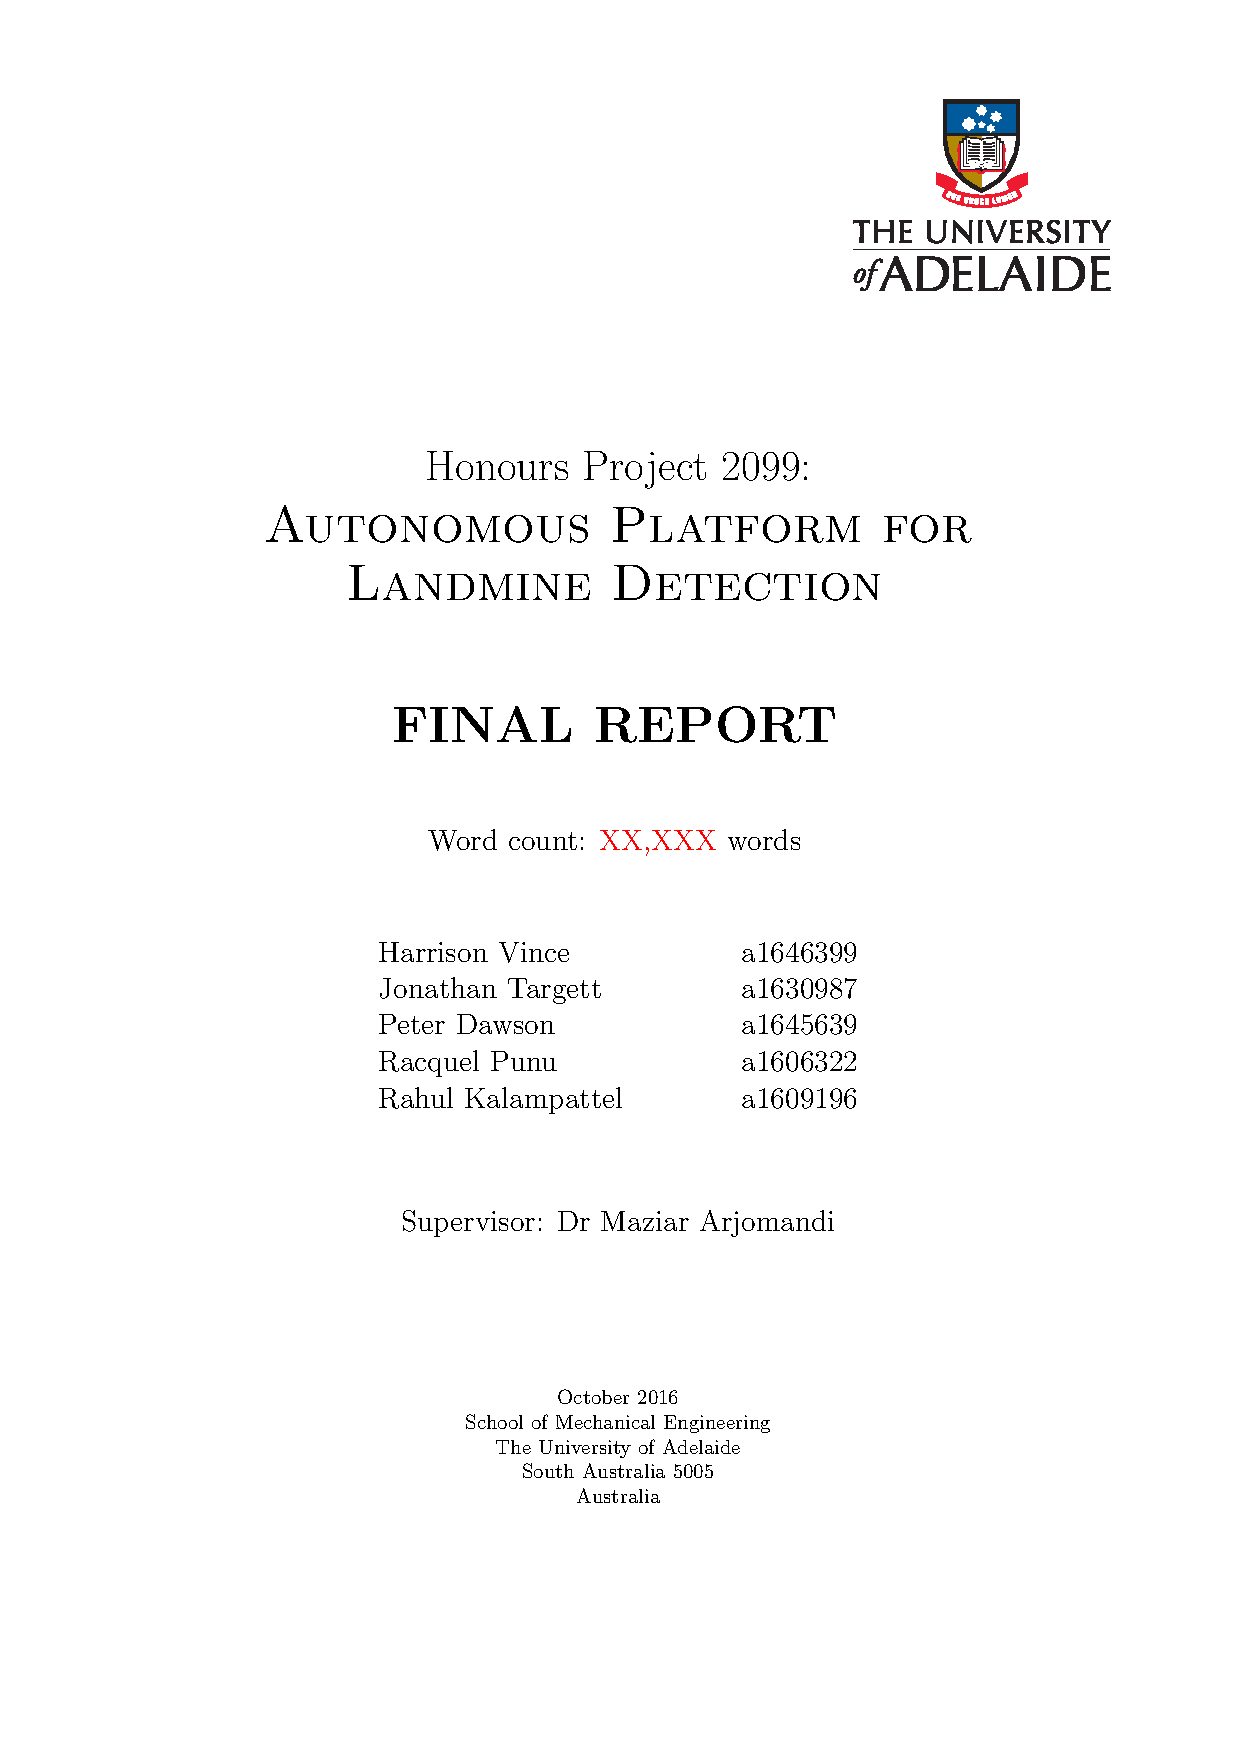
\includepdf{0-Preamble/coverpage.pdf}	% Get cover page (output from separate project)

\pagenumbering{roman}	% Numbering style for preamble
\phantomsection
\addcontentsline{toc}{chapter}{Executive Summary}	% Manually add ES to ToC
\chapter*{Executive Summary}

\textcolor{red}{\textbf{Needs to be re-written to reflect structure of current report, start with intro/background/motivation, list the objectives, methods used to achieve objectives and work done (achievements). Remember, this needs to be a summary of the REPORT, not of the project.}}\\

This report details the completed design work for Honours Project 2099: Autonomous Platform for Landmine Detection. The Defence Science and Technology Group provided the primary motivation for the project, which was to reduce the risk to Australian Defence Force personnel who are tasked with demining activities. Therefore, the goal for this project is to develop and test an autonomous and unmanned multi-sensor system for landmine detection with false positive reduction. \todo[inline]{This is an in-line TODO comment}

The scenario of operations highlights the basic system requirements for both the platform and sensor equipment. The resultant operating conditions are chosen to be flat ground with dry, loose, sandy soil containing no vegetation or obstructions. Benchmarking and literature reviews highlighted the current available technologies for the necessary subsystems, primarily platform options, automation techniques, navigation and landmine detection methods. Challenges associated with the project were landmine identification with multi-sensor systems from raw data automation issues arising from waypoint navigation due to the limitations of path tracking.  

A DSTG supplied quad bike is chosen the platform as it satisfied all predefined requirements, as well as having a pre-existing remote control system installed.
%as it has an existing remote control system, reducing project risk and development time. \textcolor{red}{this is the reason it was chosen over a tracked vehicle. it was mainly chosen because it satisfied all the requirements. Its probably fine but could also consider something like: ...chosen as our platform as it excelled in all platform requirements and also had an existing remote control system pre insta.......} \textcolor{blue}{A DSTG supplied quad bike is selected as the platform as it excelled in all platform requirements benchmarked against the project's primary objectives...... - (Should be after the primary objectives, which should be somewhere after the  }

Path tracking is conducted through the pure pursuit method which excels at path tracking for low driving speeds and discontinuous curvatures, which are expected to be traversed by the platform.
The platform automation is conducted through with use of PID control to ensure accurate system control. Landmine detection is achieved through the use of Ground penetrating radar and a metal detector array supplied by the DSTG. Scanning algorithms and metrics were developed to identify and classify landmines with a percentage likelihood of them being a landmine. This was achieved by extensive tests with mimic landmines and expected clutter items to minimise the false positive rates. 
The electronics required to integrate all systems and provide the control and necessary processing power are compromised of two main components: microcontrollers and desktop computing equipment. 
The microcontrollers were chosen to handle the low level input and output automation functions, while the desktop computing equipment acts as the central software location handling all the intensive computational processing. 
Various sensor mount designs were explored with the aim to provide minimal signal interference and maximise signal to noise ratios for the detection equipment. 
The final design adheres to both sensor system requirements with all metallic objects 450 mm away from the metal detector and the GPR as close to the ground as possible. 
The mount is constructed out of structural pine and supported with vertical steel square rod section. The metal detector is fixed to the mount using nylon rods and the mount for the GPR is able to rotate in the event it hits an object so as to limit the damage it may experience. Vibrational and structural analysis were conducted on the frame and it was found that there would be no vibrational interference from the quad bike operation on the sensors. The harmonic frequency for the sensor mount was found to be 20.97 Hz and the operation frequency for the quad bike was found to be \textcolor{red}{XX Hz} 

Testing of all electrical subsystems on the Quad bike resulted in upgrades to the brakes, steering and wheel encoder. Full system testing was conducted to find the limits of the quad bike hardware. The virtual platform was constructed to allow for navigation and system testing in a safe environment, it also provided an interactive display for the tablet control unit. Remote control of the paltfrom was achieved and resulted in fine tuning of the electrical control subsystems, namely the brake and throttle responses. It was found that the braking actuator was too slow to stop the quad bike in the required distance from an operational speed of 5 km/h. Communication difficulties resulted in unpredictable behaviour from the arduino and resulted in safety concerns. Full automation testing with the sensory system attached was not completed for safety concerns. 

Project management provides a high level overview of various management aspects of the project. All primary objectives for the project were completed while the two of the three extension objectives were not fully completed. The uncompleted objectives include, manual marking of landmines and a live video feed.



 

% This document is a proposal for Honours Project 2099: Autonomous Platform for Landmine Detection. The main objective of this project is to develop and test a multi-sensor system for landmine detection, to be mounted on a mobile platform; a secondary objective is to design a framework for the automation of this platform. It is intended that this project will serve as a technology demonstrator for the next generation of autonomous landmine detection systems. 

% The key stakeholders are introduced, with a description of the required roles for each individual. These include their high-level roles and responsibilities. 

% The primary project goals are then listed, these being the tasks which shall be completed in order for the project to be deemed a success. Extended goals are also suggested; these may be difficult or outside the scope of the project, but should be undertaken if time permits after the completion of the primary goals. Both of these are to be measured against the project specifications. The deliverables listed are those items which shall be produced over the course of the project, including reports and presentations, which demonstrate that progress has been made in achieving the goals. 

% The various hardware and software resources required for the completion of the project are outlined. A work breakdown of the project then follows, where these resources, as well as human resources, are assigned to various tasks. This information is also presented on a Gantt chart, which provides a timeline for the completion of the project. Together, these two items make up the research plan. 

% Finally, a preliminary estimate of the budget for the project is made. Based on this estimate, potential sponsorship in excess of \$X,XXX will be required in order for the project goals to be feasible.

\newpage
\phantomsection
\addcontentsline{toc}{chapter}{Disclaimer}	% Manually add ES to ToC
\chapter*{Disclaimer}
As the authors of this report, we declare that the material contained within is entirely our own work, unless otherwise specified. All work from other sources has been referenced accordingly. 
\vspace{0.4in}

% Update with correct images for signatures when ready, change dates as well

\noindent\begin{tabular}{ll}
\raisebox{-0.4in}[0pt][0pt]{
\includegraphics[height=0.7in]{0-Preamble/Harry.png}}&\raisebox{-0.0in}{24/10/2016}\\
\makebox[2.5in]{\hrulefill} & \makebox[1.4in]{\hrulefill}\\
Harrison Vince & Date\\[0.4in]% adds space between the two sets of signatures
\raisebox{-0.4in}[0pt][0pt]{
\includegraphics[height=0.7in]{0-Preamble/Harry.png}}&\raisebox{-0.0in}{24/10/2016}\\
\makebox[2.5in]{\hrulefill} & \makebox[1.4in]{\hrulefill}\\
Jonathan Targett & Date\\[0.4in]% adds space between the two sets of signatures
\raisebox{-0.4in}[0pt][0pt]{
\includegraphics[height=0.7in]{0-Preamble/Harry.png}}&\raisebox{-0.0in}{24/10/2016}\\
\makebox[2.5in]{\hrulefill} & \makebox[1.4in]{\hrulefill}\\
Peter Dawson & Date\\[0.4in]% adds space between the two sets of signatures
\raisebox{-0.4in}[0pt][0pt]{
\includegraphics[height=0.7in]{0-Preamble/Harry.png}}&\raisebox{-0.0in}{24/10/2016}\\
\makebox[2.5in]{\hrulefill} & \makebox[1.4in]{\hrulefill}\\
Racquel Punu & Date\\[0.4in]% adds space between the two sets of signatures
\raisebox{-0.4in}[0pt][0pt]{
\includegraphics[height=0.7in]{0-Preamble/Rahul.jpg}}&\raisebox{-0.0in}{24/10/2016}\\
\makebox[2.5in]{\hrulefill} & \makebox[1.4in]{\hrulefill}\\
Rahul Kalampattel & Date
\end{tabular}
\newpage

\phantomsection
\addcontentsline{toc}{chapter}{Acknowledgements}	% Manually add ToC to ToC
\chapter*{Acknowledgements} 
The authors of this report acknowledge the contribution of several parties, without whom this project would not have been possible.

Firstly, the authors would like to thank the project sponsor, the Defence Science and Technology Group. As well as providing funding and equipment, the technical insights shared by Dr Canicious Abeynayake and his colleagues of the Weapons Effects \& Protection group are greatly appreciated. 

The authors also acknowledge the help of Kyle Blay from CSIRO and Greg Harmer from Minelab, both of whom provided invaluable assistance in understanding the sensor systems.

At the University of Adelaide, Rob Dempster, Phil Schmidt and several other members of both the Mechanical Engineering and Electronics and Instrumentation Workshops were responsible for helping out on numerous occasions. The authors also thank Marc Simpson at Thebarton Labs for allowing the use of lab facilities. 

Finally, the authors would like to thank Dr Maziar Arjomandi, the project supervisor, for his guidance and feedback throughout the year. 
\newpage

\phantomsection
\addcontentsline{toc}{chapter}{Contents}	% Manually add ToC to ToC
\renewcommand{\baselinestretch}{1.2}\normalsize 	% 1.2 line spacing
\tableofcontents
\renewcommand{\baselinestretch}{1.3}\normalsize 	% 1.3 line spacing
\newpage

\phantomsection
\addcontentsline{toc}{chapter}{List of Figures}	% Manually add LoF to ToC 
\listoffigures
\newpage

\phantomsection
\addcontentsline{toc}{chapter}{List of Tables}	% Manually add LoT to ToC
\listoftables
\newpage

% Uncomment the three lines below to split nomenclature into two columns
% \renewcommand*{\nompreamble}{\begin{multicols}{2}}
% \renewcommand*{\nompostamble}{\end{multicols}}
% \setlength{\columnsep}{3em}

\printnomenclature
\newpage

\end{document}